%---------change this for every latex homework
\def\yourid{rtg5xkh}
\def\collabs{}
\def\sources{Cormen, et al, Introduction to Algorithms.}
% -----------------------------------------------------
\def\duedate{Tuesday,  May 3, 2022 at 11:30 pm }
\def\duelocation{via Gradescope}
\def\htype{Adv}
\def\hunit{D}
\def\hnumber{}
\def\course{{cs4102 - algorithms - spring 2022}}%------
%-------------------------------------
%-------------------------------------

\documentclass[10pt]{article}
\usepackage[colorlinks,urlcolor=blue]{hyperref}
\usepackage[osf]{mathpazo}
\usepackage{amsmath,amsfonts,amssymb, graphicx}
\usepackage{latexsym}
\usepackage[top=1in,bottom=1.4in,left=1.25in,right=1.25in,centering,letterpaper]{geometry}
\usepackage{color}
\definecolor{mdb}{rgb}{0.1,0.6,0.4} 
\definecolor{cit}{rgb}{0.05,0.2,0.45} 
\pagestyle{myheadings}
\markboth{\yourid}{\yourid}
\usepackage{clrscode}
\usepackage{tabularx}
\newcolumntype{Y}{>{\centering\arraybackslash}X}

\usepackage{framed}

\newenvironment{proof}{\par\noindent{\it Proof.}\hspace*{1em}}{$\Box$\bigskip}
\newcommand{\handout}{
   \renewcommand{\thepage}{Unit \hunit: \htype~Homework \hnumber~-~\arabic{page}}
   \noindent
   \begin{center}
      \vbox{
    \hbox to \columnwidth {\sc{\course} \hfill}
    \vspace{-2mm}
       \hbox to \columnwidth {\sc due \MakeLowercase{\duedate} \duelocation\hfill {\Huge\color{mdb}\hunit\hnumber{\Large\MakeLowercase{\htype}}(\yourid)}}
      }
   \end{center}
   \vspace*{1mm}
   \hrule
   \vspace*{1mm}
    {\footnotesize \textbf{Collaboration Policy:} You are encouraged to collaborate with up to 3 other students, but all work submitted must be your own {\em independently} written solution. List the computing ids of all of your collaborators in the \texttt{collabs} command at the top of the tex file. Do not share written notes, documents (including Google docs, Overleaf docs, discussion notes, PDFs), or code.  Do not seek published or online solutions for any assignments. If you use any published or online resources (which may not include solutions) when completing this assignment, be sure to cite by naming the book etc.\ or listing a website's URL. Do not submit a solution that you are unable to explain orally to a member of the course staff. Any solutions that share similar text/code will be considered in breach of this policy. Please refer to the syllabus for a complete description of the collaboration policy.
   \vspace*{1mm}
    \hrule
    \vspace*{2mm}
    \noindent
    \textbf{Collaborators}: \collabs\\
    \textbf{Sources}: \sources}
    \vspace*{2mm}
    \hrule
    \vskip 2em
}

\newcommand{\solution}[1]{\color{blue}\hfill\break\noindent\textbf{Solution:} #1\color{black}}

%\newcommand{\solution}[1]{}
\newcommand{\altsolution}[1]{}

\newcommand{\bit}[1]{\{0,1\}^{ #1 }}
%\dontprintsemicolon
%\linesnumbered
\newtheorem{problem}{\sc\color{cit}problem}
\newtheorem{practice}{\sc\color{cit}practice}
\newtheorem{lemma}{Lemma}
\newtheorem{definition}{Definition}
\newtheorem{theorem}{Theorem}

\newcommand{\Z}{\mathbb{Z}} % This might be useful for Integers!

\begin{document}
\thispagestyle{empty}
\handout

%----Begin your modifications here


\begin{problem} IKEA Grill \end{problem}
IKEA is growing in popularity across the US, however their stores are only found in a handful of larger metropolitan areas.  While their main product is furniture, they have become known for their signature meatballs.  To increase profits and make their delicious food more accessible, they have decided to open local IKEA Grill restaurants in towns across the country.  Restaurant storefronts are expensive to rent and maintain, so they are happy with customers needing to drive at most to the next town over to get their IKEA meatball fix.  Specifically, their goal is that every town in America either has an IKEA Grill, or its neighboring town has an IKEA Grill.

Given a graph representing the towns (as vertices) and roads between them (edges connecting neighboring towns), the \emph{IKEA Grill} problem is to decide whether $k$ IKEA Grill locations can be placed in order to ensure that each town or its neighbor has an IKEA Grill location.  Show that \emph{IKEA Grill} is NP-Complete.

Note: You are not being asked to explicitly solve the \emph{IKEA Grill} problem; you are only required to show that it is NP-Complete.

\solution{
    To show that this is NP-Complete, first we will show that it is NP. \\
    We can do this by proving that a potential solution to the \emph{IKEA Grill} problem can be checked in polynomial time. Given a graph representing all towns as vertices and all neighboring towns having an edge between them, with k vertices "selected" as locations for IKEA Grills, we can verify the solution as follows: traverse through each vertex of the graph using BFS, and for each of these vertices, verify that either that vertex is "selected" or one of it's neighbors is "selected" (BFS naturally looks at a vertex and then all of its neighbors). If every vertex has this property, the proposed solution is correct. If not, it is not a valid solution. This verification will have a polynomial runtime, thus the problem is in NP. \\
    Next, we will show that the problem is NP-Hard. From lecture we know that the k-Vertex Cover Problem is NP-Hard. Thus if we can reduce it to the IKEA Grill problem, we will have proven that the IKEA Grill problem is NP-Hard. \\ 
    Given an input to the k Vertex Cover Problem, if we can convert that input somehow, run the IKEA Grill problem on it, and return a result that's always the same as the true answer to the k-Vertex cover problem, then we will have proven the IKEA Grill problem is NP-Hard. That is, we must reduce the k-Vertex cover problem to the IKEA Grill problem. \\
    We can do this by altering the input graph for the k-Vertex cover problem in the following manner: \\
    (1) if there exist any isolated nodes in the graph (i.e. a vertex with no edges that connect to it), remove them. This is necessary because k-vertex cover would never select these nodes - they don't help cover the edges. \\
    (2) For each edge $e_i$ in the graph that connects 2 nodes which we'll call $n_1$ and $n_2$, we will add 2 edges and 1 more node to the graph, where one new edge will connect $n_1$ to the new node, and the other new edge will connect $n_2$ to the new node. For each edge in the graph the conversion will look like this: \\
    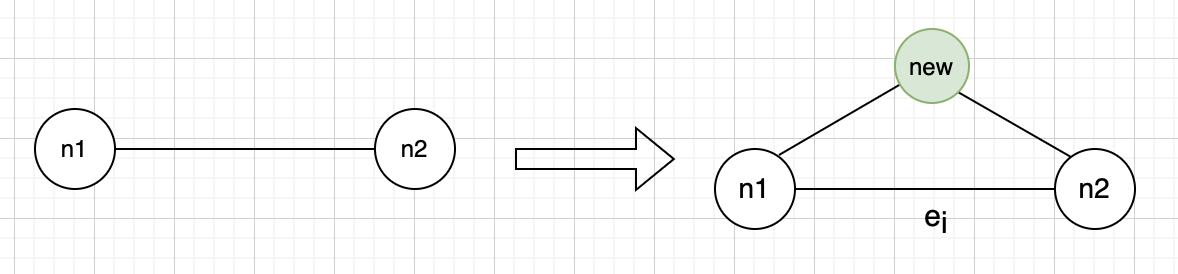
\includegraphics[scale=.8]{ikea.png}
    Intuitively, it makes sense that for this conversion we would need to add more edges and vertices to the graph to be used as input to the IKEA Grill problem because the IKEA grill problem has more "flexibility". By this, I mean that its coverage of the graph doesn't need to be as extensive as the coverage must be for the k-vertex cover problem because it simply needs to cover every vertex or its neighbor, and can do this without actually covering each edge (which k-vertex requires). \\
    This is essentially the problem we need to solve with this conversion: Given a certain graph input to k-vertex cover, how can we convert it such that, if the the IKEA Grill problem returns true on the converted graph for the same k, the k-vertex cover problem \emph{would have} returned the same result. The two problems are very similar, and the difference lies in the fact that, if given the \emph{same} graph input, the IKEA grill problem could devise a set of vertices that solve its own problem, but do not cover some edges in the graph. To eliminate this discrepancy, we will employ the strategy described above. The new node added will force each edge $e_i$ that was present in the original graph to be covered by one of its two nodes in the IKEA Grill solution. For example, considering the example above, the new node will force either n1 or n2 to be selected by IKEA grill, because otherwise the new node will not be covered. The new node itself would not be selected by IKEA grill unless n1 and n2 did not connect to any other nodes in the original graph. In this case, it wouldn't matter because regardless of which of the 3 nodes in this "triangle" were selected, the answer would not change. It's also important to note that we of course assume that n1 and n2 may (and probably will) be connected to other nodes that were in the original graph (not shown in the image). When they are connected to other actual nodes in the graph, this conversion and answer will still work because each of those other nodes in the graph will also have a 'new' node that they will be connected to, forcing each original edge in the whole graph to be covered. \\
    We can iterate through each edge in the graph in a time complexity related to the number of edges, and we can add the new node and 2 edges in constant time. Thus, the graph conversion can be done in polynomial time. \\
    We have crafted an implementation of the k-vertex cover problem using only the IKEA Grill problem and a polynomial time reduction involving a conversion of the graph. Since k-vertex is NP-Hard and we reduced it to IKEA Grill, it must be true that the IKEA Grill problem is also NP-Hard. \\
    Therefore IKEA Grill is NP-Complete because we have proven it is both NP and NP-Hard.
}


\begin{problem} Backpacking, Revisited \end{problem}
After your first successful backpacking adventure (Unit C's Advanced, Problem 1), you have decided to return to
Shenandoah National Park. Similar to before, you and your friend have completed your packing list, and you need
to bring $n$ items in total, with the weights of the items given by $W = (w_1, \ldots, w_n)$. Your goal
this time is to divide the items between the two of you such that the difference in weight is as small as possible.
There is no longer a restriction on the total number of items that each of you should carry.
Here, we will define a decisional version of this \textsc{Backpacking} problem:
\begin{framed}
  \noindent
  \textsc{Backpacking}: Given a sequence of non-negative weights $W = (w_1, \ldots, w_n)$ and a target weight difference
  $t$, can you divide the items among you and your friend such that the weight difference between backpacks is at most $t$?
\end{framed}
\begin{enumerate}
  \item Show that the \textsc{Backpacking} problem defined above is $\mathsf{NP}$-complete (namely, you should
  show that $\textsc{Backpacking} \in \mathsf{NP}$ and that \textsc{Backpacking} is $\mathsf{NP}$-hard). For this
  problem, you may use the fact that the \textsc{SubsetSum} problem is $\mathsf{NP}$-complete:

  \begin{minipage}[t]{\linewidth}
  \begin{framed}
    \textsc{SubsetSum}: Given a sequence of non-negative integers $a_1, \ldots, a_n$
    and a target value $t$, does there exist
    a subset $S \subseteq \{ 1, \ldots, n \}$ such that $\sum_{i \in S} a_i = t$?
  \end{framed}
  \end{minipage}
  
  \solution{
    First, we will show that \textsc{Backpacking} is NP: \\
    Given a potential answer to the problem (which is two sequences of the weights), we can check if it is correct in linear time. We will simply take the sum of each sequence, and compare the difference between those two sums to $t$. If it is greater than $t$, the division of items is not valid. Else, it is valid. Since we are able to verify a possible  solution in polynomial time, \textsc{Backpacking} is in NP. \\
    Next, we will show that it is NP-Hard: \\
    To do this, we will prove that \textsc{SubsetSum} reduces to \textsc{Backpacking} in polynomial time. \\
    To do this reduction, first we will take the sum of all numbers in \textsc{SubsetSum}'s input sequence, which we'll call $sum_s$ (We'll also choose to call the input sequence $seq_{ss}$. We will also make use of $t$ (the other input to \textsc{SubsetSum}) to add some additional weights to the input for \textsc{Backpacking}. \\ The idea is that we will need to carefully select our inputs to the backpacking problem such that the only possible way it will return true is when there existed some subset of $seq_{ss}$ whose sum was equal to t. We will convert the input as follows: \\
    All of the numbers in $seq_{ss}$ will be part of W (an input to \textsc{Backpacking}), and we will add two additional weights to W: $2sum_s - t$ and $sum_s + t$. The reasoning for these two additions to the will be obvious later on. We will also use $0$ for the second input to \textsc{Backpacking}, and we'll call this input $diff$ instead of $t$ (we will continue to use $t$ to identify the original target input to \textsc{SubsetSum}). $diff$ \emph{must} be $0$ for the conversion from SubsetSum to \textsc{Backpacking} to work. This is because for \textsc{SubsetSum}, the answer requires a subset to be \emph{exactly} equal to t, whereas for \textsc{Backpacking}, it will return true if a division of weights can result in a difference \emph{less than or equal to} $diff$. This distinction is important, and since a difference cannot be less than $0$, by choosing $diff = 0$, we ensure that the only way \textsc{Backpacking} will return true is if there can be a division of weights such that the weight carried by the two people, p1 and p2, is equal. By doing this we also remove the "less than or equal to" part of the \textsc{Backpacking} problem, because a difference cannot be less than $0$ so $0$ is now the only option for the difference. \\
    Our set of weights will look like this: \\
    $W = (w_1, \ldots, w_n, 2sum_s - t, sum_s + t)$ \\
    Where $w_1$ through $w_n$ are the same as $a_1$ through $a_n$ from the \textsc{SubsetSum} input. With this set of weights and $diff = 0$, if \textsc{Backpacking} returns true on this input, it must have been true that some subset of $seq_{ss}$ had a sum equal to $t$ \textsc{SubsetSum}. \\ 
    To prove this, we will first take advantage of the fact that every weight will be assigned to one of the two people. Consider the assignments of the weights in $w_1$ through $w_n$. One subset of them will be assigned to $p1$, and the other will be assigned to $p2$. Let's say $X$ is the sum of the subset of weights in $w_1$ through $w_n$ that are assigned to $p1$. Thus, the subset of weights in $w_1$ through $w_n$ that are assigned to $p2$ must be $sum_s - X$. Considering the fact that we have another weight $2sum_s - t$, and another one with $sum_s + t$, for the weights to be evenly distributed between the two people , we will want to assign $2sum_s - t$ to $p1$ and and $sum_s + t$ to $p2$ (because we need the 4 total $sum_s$'s present to be split 2 and 2 between the people). We are left with these totals: \\
    $p1: X + 2sum_s - t$ \\
    $p2: sum_s - X + sum_s + T$ \\
    We must make these equal if we are to fulfill the requirement $diff = 0$. \\
    \begin{align*}
        X + 2sum_s - t &= 2sum_s - X + t \\
        X - t &= -X + t \\
        2X &= 2t \\
        X &= t
    \end{align*}
    We have proven that the only possible way for the difference between the two weights to be $0$ (which is the case where \textsc{Backpacking} returns true) is if $X = t$, where $X$ is a subset of $seq_{ss}$. This is the answer to \textsc{SubsetSum} that we were originally seeking, so we have implemented \textsc{SubsetSum} using \textsc{Backpacking}. Since we simply must take the sum and add two weights, the reduction will be linear and thus is polynomial-time. We have proven that an NP-Hard problem, \textsc{SubsetSum}, can be reduced to \textsc{Backpacking}, thus \textsc{Backpacking} is NP-Hard. \\
    Since \textsc{Backpacking} is both in NP and NP-Hard, it must be NP-Complete.
  }

  \item Your solution to Unit C Advanced's Problem 1 can be adapted to solve this version of the \textsc{Backpacking} problem
  in time that is {\em polynomial} in $n$ and $M$, where $M = \max(w_1, \ldots, w_n)$ is the maximum weight of all of the items. Why did this
  not prove $\textsf{P} = \textsf{NP}$? ({\em Conversely, if you did prove that $\textsf{P} = \textsf{NP}$, there's a nice
  check waiting for you at the \href{https://www.claymath.org/millennium-problems/p-vs-np-problem}{Clay Mathematics Institute}.})
  
  \solution{
    The reason for this is because while the time complexity appears to be polynomial in terms of M and n, it's not actually polynomial (it's pseudo-polynomial). Since M is a natural number, it will actually need to be represented in terms of the number of bits, and using this input size the time complexity will technically be exponential. Since the runtime was not actually polynomial this solution does not prove P = NP.
  }
\end{enumerate}


\begin{problem} Gradescope Submission \end{problem}
Submit a version of this \verb|.tex| file to Gradescope with your solutions added, along with the compiled PDF.  You should only submit your \verb|.pdf| and \verb|.tex| files.


\end{document}

